\section{Technische Funktionsweise von Bitcoin}
\label{sec:mechanics}

Mithilfe dieser kryptografischen Mechanismen lässt sich ein Zahlungsnetzwerk aufbauen, in welchem --~im Gegensatz zu herkömmlichen Banken~-- keine zentrale vertrauenswürdige Stelle notwendig ist.
Wie sich der Stand eines Kontos aus vorangegangen Transaktionen ergibt, so setzt sich auch der Kontostand einer Bitcoinadresse aus vorhergegangen Transaktionen statt.
Da es keine zentrale Stelle gibt und das Guthaben jeder Adresse daher öffentlich verfügbar sein muss, müssen auch alle Transaktionen öffentlich gemacht werden.

\subsection{Transaktionen}

\begin{figure}
    \begin{center}
        \includegraphics[page=2,trim={62mm 168mm 62mm 56mm},clip,scale=1.2]{data/figures/bitcoin.pdf}
    	\caption{Unverzweigte Transaktionskette \parencite[2]{nakamoto}}
    	\label{fig:transactionchain}
    \end{center}
\end{figure}

\begin{figure}
    \begin{center}
        \includegraphics[page=5,trim={88mm 59mm 88mm 195mm},clip,scale=1.2]{data/figures/bitcoin.pdf}
    	\caption{Transaktion mit mehreren Aus- und Eingängen \parencite[5]{nakamoto}}
    	\label{fig:transaction}
    \end{center}
\end{figure}

Transaktionen sind wohl der wichtigste Bestandteil des Bitcoin-Netzwerks.
Denn anstatt einen Kontostand zu speichern und ihn bei jeder Transaktion zu verändern (was anfällig für Manipulation wäre), beziehen sich Transaktion auf vorhergegangene Transaktionen, damit die Herkunft und somit die Gültigkeit verifiziert werden.
Eine Transaktion kann dabei aus mehreren Eingängen und mehreren Ausgängen bestehen.
Ein Eingang referenziert dabei immer einen Ausgang einer Vorherigen Transaktion, welcher dann vollständig aufgebraucht werden muss.
Möchte man nur einen Teil der Bitcoins aus dem alten Ausgang ausgeben, so muss es zwei Ausgänge geben, wobei einer einen Teil an eine Andere Adresse sendet und der andere den Rest wider zurück an einen selbst.



\subsection{Adressen}

Mithilfe der Bitcoinadressen wird gewährleistet, dass nur autorisierte Personen die Ausgänge vergangener Transaktionen als Eingang in ihrer Transaktion verwenden können.
Bei den Adressen handelt es sich genaugenommen um ein asymmetrisches Schlüsselpaar, mit dem Transaktionen signiert werden, wobei der öffentliche Schlüssel als Adresse zum Empfangen von Bitcoins dient.
Erstellt man eine Transaktion, so referenziert man im Ausgang den öffentlichen Schlüssel des Empfänger der Bitcoin.
Möchte dieser die Bitcoin nun weitergeben so muss er diesen Ausgang in dem Eingang seiner Transaktion referenzieren.
Anschließend bildet er den Hashwert der Transaktion und signiert diesen mit seinem privaten Schlüssel.
Somit ist von jedem nachvollziehbar, dass es sich beim Ersteller der Transaktion um den Inhaber der Bitcoins handelt, indem man die Signatur mit dem öffentlichen Schlüssel aus der vorhergegangen Transaktion überprüft.

Diese öffentliche Nachvollziehbarkeit ist der Schlüssel in der Funktionsweise von Bitcoin.
Erst durch die aus der asymmetrischen Verschlüsselung folgenden Signaturen ist es möglich den Urheber einer Transaktion ohne eine zentrale Vertrauensstelle zu überprüfen.

\subsection{Die Blockchain}

\begin{figure}
    \begin{center}
        \includegraphics[page=3,trim={66mm 179mm 66mm 81mm},clip,scale=1.2]{data/figures/bitcoin.pdf}
    	\caption{Vereinfachte Darstellung der Blockchain \parencite[3]{nakamoto}}
    	\label{fig:blockchain}
    \end{center}
\end{figure}

Um die Transaktion zu speichern werden mehrere Transaktion in sogenannte \emph{Blocks} zusammengefasst.
Da jeder Block neben den Transaktionen auch eine Referenz in Form des Hashes auf den vorherigen Block beinhaltet, entsteht eine lineare Kette von Blöcken -- \emph{Blockchain} genannt.
Aufgrund der Linearität der Blockchain kann gewährleistet werden, dass jeder Transaktions-Ausgang nur einmal von einem Eingang aufgegriffen wird und somit sogenannten \emph{Double-Spending} (d.h. das zwei- oder mehrmalige Verwenden eines Ausganges in verschiedenen Transaktionen) verhindert wird.

\subsubsection{Mining}
\label{subsec:mining}

Unter \emph{Mining} versteht man das generieren von Blöcken.
Da man möchte das Blöcke nur so langsam erschaffen werden, dass sich das Bitcoin-Netzwerk über einen gemeinsamen aktuellen Block einig ist, ist ein gewisser Aufwand mit der Erstellungen eines Blockes verbunden.
Diese \emph{Proof-of-Work}-Mechanismen sorgen dafür, dass durchschnittlich nur alle 10 Minuten ein neuer Block erzeugt wird.

Hierzu erstellt eine \emph{Mining-Software} einen temporären Block aus bestehenden, noch nicht in der Blockchain vorhandenen Transaktionen.
Dann berechnet sie den Hashwert des Blockes und vergleicht ihn mit dem Ziel-Wert.
Ist der Hash kleiner als der Zielwert, handelt es sich um einen gültigen Block.
Sollte der Hash größer sein, so gibt es einen 32-Bit großen Teil des Blockes (\emph{Nonce} genannt), welcher nach belieben verändert werden kann, um einen entsprechenden Hash zu erhalten.
Da sich der Hash scheinbar zufällig ändert, muss der Miner relativ viele Hashwerte berechnen, bis er einen gültigen findet.
Der Zielwert wird anhand einer Formel alle zwei Wochen angepasst, damit egal wie viel Mining betrieben wird, immer durchschnittlich alle 10 Minuten ein gültiger Block gefunden wird.

Um die Miner für die aufgewandte Rechenleistung und Stromkosten zu entschädigen, ist in jedem Block eine Transaktion enthalten, in der der Miner einen gewissen Betrag erhält, den es vorher nicht gab.
Über diesen Weg funktioniert auch die Wertschöpfung des Bitcoin-Netzwerkes.
Die erschaffene Belohnung für das Mining betrug am Anfang 50 Bitcoins pro Block, wird aber alle 210000 Blöcke (alle 4 Jahre) halbiert, so dass Bitcoin trotz dauerhafter Zufuhr auf ein Maximum von 21 Millionen Bitcoins limitiert ist.
Außerdem können Miner die Differenzen zwischen Eingang und Ausgang in Transaktionen, die sie in ihrem Block einschließen behalten.

Aufgrund dieser Eigenschaften kann Mining profitabel sein, wenn der Wert der erhaltenen Bitcoins über dem der Anschaffungs und Betriebskosten der Mining-Hardware liegt.
Während es in den Anfängen von Bitcoin profitabel war, mit herkömmlichen Prozessoren Mining zu betreiben, welche zirka einige Millionen Hashwerte pro Sekunde berechnen können wurde bald durch die hohe Anzahl der Miner der Zielwert niedriger und es somit nicht mehr profitabel.
Da Grafikkarten für manche Rechenoperationen schneller sind als Prozessoren wurden darauf diese verwendet, womit fast eine Milliarde Berechnungen pro Sekunde möglich wurden.
Seit Ende 2012 gibt es auch dezidierte Mining-Hardware, welche nur dazu gebaut wird, Bitcoin-Mining zu betreiben.
Mit dieser Hardware sind inzwischen Geschwindigkeiten von bis zu 8~THash/s (8~Billionen Hashwertberechnungen pro Sekunde) möglich.

\subsubsection{Linearität}

Sollte es einmal vorkommen, dass ein Miner einen Block findet, bevor er den aktuellsten Block vom Bitcoin-Netzwerk erhalten hat, kommt es zu einer Verzweigung der Blockchain.
Hierbei kann es vorkommen, dass dieselben Bitcoins in jedem der Blöcke an verschiedene Empfänger gesendet werden.
Um zu verhindern, dass man somit Bitcoins verdoppeln kann, darf nur einer der zwei gleichzeitig generierten Blöcke weiterverwendet werden, während der andere für ungültig erklärt wird.
Die Auswahl des ungültigen Blocks geschieht gewissermaßen durch Zufall.
Während jeder Bitcoin-Client und jeder Miner zuerst den Block verwendet, den er als erstes erhalten hat, werden sich alle Beteiligten über einen Block einig, sobald ein Miner den nächsten Block findet, egal, welcher der beiden Blöcke als Ursprung dient.
Die in dem jetzt ungültigen Block gelisteten Transaktionen sind somit noch nicht verifiziert worden und werden in die nächsten Blöcke aufgenommen.
